\chapter{State of the art short-term residential load forecasting techniques}
\label{cha:State of the art short-term residential load forecasting techniques}
Forecasting the electrical load of the different individual households has a couple of challenges. There should be dealt with the missing values, as discussed in section \ref{s:missing_data}. Also, the different time-series are influenced by exogenous factors as weather conditions and the day of the year. The dependency on exogenous variables can be a very non-linear relation and can have different effects on different households. For example depending on a house has solar panels, the consumption could be altered much. Only three indications of the temperature are given on a daily basis. Some additional information is know of certain households, but this data is very incomplete. Next, the individual load series have a high volatility and uncertainty with respect to a load signal on transmission level which shows more consistent seasonality and straight forward dependency on weather and calendar variables. This is because the contingency of the individual load data is mitigated due to averaging out of the uncertainty. Ofcourse, the obvious disadvantage is that only forecasts on this aggregated level can be made which is not the goal of our investigation.\\ To tackle the high non-linearity that is inherent to residential load forecasting in literature often ``Neural Networks'' are used.
\textbf{See also paper TA2 --> aggregated vs individual forecasting.}

\section{Introduction to Neural Networks}\label{s:Introduction to Neural Networks}
A  standard multilayer feedforward neuralnetwork with locally bounded piecewise continuous activation function can approximate any continuous function to any degree of accuracy if and only if the network's activation function is not a polynomial, as stated by \textbf{Leshno et al} in \textbf{1993}. This theorem proofs that a ``universal approximator'' exists for continuous functions, but it lacks the recipe to construct it. In \cite{Nielsen2015} it is shown that a feedforward network with a single layer is enough to approximate any function by a specified accuracy if the hidden layer has the possibility to add an unlimited amount of hidden neurons in its layer. It is discussed that when a function is discontinuous, which means that it makes sudden, sharps jumps, it is not possible to approximate the function by any prescribed accuracy. However, in practise a continuous approximation is often good enough.\\

Neural networks are suitable of learning very non-linear mappings between inputs and outputs. The difference between ``Deep Neural Networks'' and ``Shallow Neural Networks'' is the amount of layers of neurons are used inside the network. These layers of neurons, that are not inputs or outputs are called ``hidden neurons''. Because a ``Deep Neural Network'' has a hierarchical layout of the different hidden layers, it not only learning features from the non-linear combinations of inputs, but uses other layers to learn features of combinations of features learned in lower hidden layers. This is possible because higher hidden layers get the outputs of lower hidden layers as input. As discussed in  \cite{Shi2018} due to this characteristic, deep learning is suitable to learn multiple uncertainties with differing sharing levels over different households e.g. the amount of sunshine. However, because of the higher expressiveness (and often the amount of the to learn parameters), a ``Deep Neural Network'' with respect to a ``Shallow Neural Network'', suffers more of overfitting as is discussed in section \ref{s:Problems}.

\subsection{MLP}
The simples configuration of deep networks are multilayer perceptrons and they are made up out of multiple fully connected layers of neurons. Figure \ref{fig:MLP} shows a MLP with one hidden layer.

\begin{figure}[h!]
	\centering
	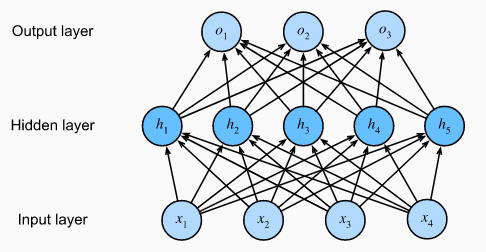
\includegraphics[width=0.8\textwidth]{MLP.png}
	\caption{Figure of a MLP (source \cite{Czum2020}).}
	\label{fig:MLP}
\end{figure}

All layers are connected to the next layer by the means of an affine function together with a non-linear activation function represented by sigma as shown by equation \ref{eq:NN} with $ \textbf{L}^{(N)} $ the vector with outputs of the Nthe layer, $ \textbf{W}^(N) $ the Nth weight matrix and $ \textbf{b}^{(N)} $ the Nth bias

%It can be noted that the MLP network is invariant.

\begin{equation}\label{eq:NN}
	\textbf{L}^{N+1} = \sigma(\textbf{W}^{(N)}\textbf{L}^{N}+\textbf{b}^{(N)}).
\end{equation}


\subsection{CNN}
\textbf{See oneNote}

\subsection{RNN}\label{s:RNN}
A recurrent Neural Network is a specialized neural network to better deal with sequential information. While traditional deep neural networks assume that inputs and outputs are independent of each other, the output of recurrent neural networks depend on the prior elements within the sequence. In order to take past information from previous inputs into account, a hidden variable $ h_t $ is used. By making use of this variable which makes a summary of the previous seen information, an exponential increase in the number of model parameters is avoided. Cited from \cite{bibid}: ``Hidden states are technically speaking inputs to whatever we do at a given step, and they can only be computed by looking at data at previous time steps''. Equation \ref{eq:RNN} shows how the previous hidden state and the current information are merged in the next hidden state with $ \textbf{X}^t\in \mathbb{R}^{d\times 1} $, $ \textbf{H}^t\in \mathbb{R}^{h\times 1} $, $ \textbf{W}_1\in \mathbb{R}^{h\times d} $, $\textbf{W}_2\in \mathbb{R}^{h\times h} $ and $ \textbf{b}\in \mathbb{R}^{h\times 1} $ 

\begin{equation}\label{eq:RNN}
	\textbf{H}^{t+1} = \tanh(\textbf{W}_1\textbf{X}^{t}+\textbf{W}_2\textbf{H}^{t}+\textbf{b}).
\end{equation}

The equation $\textbf{X}^t$ corresponds to one example at time step $ t $ with dimensionality $ d $. 
Also a deep RNN is possible, where multiple hidden state per time step are used. \\

\begin{figure}[h]
	\centering
	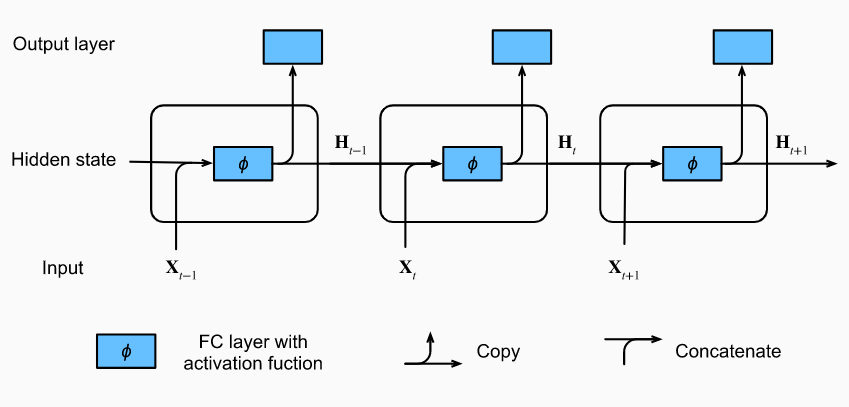
\includegraphics[width=1.0\textwidth]{RNN.png}
	\caption{Figure of the logical flow of a vanilla RNN with a hidden state (source: \cite{Czum2020}).}
	\label{fig:RNN}
\end{figure}

As was discussed in Section \ref{s:Introduction to Neural Networks} a standard neural network can act as a ``universal approximator'' when given enough hidden states. A similar result exist for a recurrent neural network which states that it is capable to approximate a sequence-to-sequence mapping to  an arbitrary accuracy as discussed in \cite{Hammer2000}. However, as discussed in \cite{Teuwen2019} even if expressiveness of the simple model is very powerful in theory, this doesn't indicate that such a representation can be learn in a reasonably amount of time from a dataset. As will be discussed in Section \ref{s:Problems}, the main drawback of the vanilla recurrent neural network is that it forgets fast, important information in function of the amount of time steps. When using ``backpropagation through time'' for updating the weights, the gradients that corresponds to inputs seen a lot of time steps ago will become very small due to the multiplication of small gradients over the time steps. Therefore, there contribution of updating the weights of the recurrent neural network will be very small and thus this information will be ``forgotten''.


\subsection{Difficulties \& Solutions of neural networks}\label{s:Problems}
Neural Networks have a high expressiveness but comes at the cost of overfitting and a vanishing gradient.
when the NN is learning from training data, every epoch the error between the input and output of the training exemples is reduced. In the beginning the generalization error reduces simultaneously with the generalization error. The generalization error is the error that the model makes on data that is not in the training set. However, on a certain point during the training the generalization error increases while the training error still decreases. This means that the model is no longer learning ``intelligent'' general rules and patterns in the data, but is just remembering the training data and will therefore not apply in general. This is often the case in a model with high expressiveness because the model is less pushed to make generalizations and has the ability to just to remember the training data. Solutions to overfitting can be regularization which includes the parameter norms as a cost in the objective function. Typical choices for resembling the size of a parameter are the $ L_1 $ and the $ L_2 $ norms. Other methods that can be used are: early stopping, dropout and pruning.

It should also be noted that the gradient can increase very much over the different time steps, which in literature is called gradient explosion. The solution strategy for this is applying gradient clipping by norm or by value. Gradient clipping by norm means that when the two norm of the gradient $ \bm{\xi} $ exceeds a threshold value $ \theta $, the two norm of the gradient is scaled to equal the threshold value. The mathematical formulation is given by equation \ref{eq:clipping}:

\begin{equation}\label{eq:clipping}
	\bm{\xi}= min(1,\frac{\theta}{\| \bm{\xi} \|})\times\bm{\xi}.
\end{equation}


The second problem is the vanishing gradient problem which originates because while using the backpropagation algorithm to calculate the gradient which is used in different update methods of the weights, the gradient is calculated at the end of the NN and propagated back using every time the previous calculated gradient values which exponentially decreases in function of the time steps. Therefore, at the first layers of the network, the gradient has become so small that the weights are almost not updated anymore. In a RNN setting this corresponds to having a short term memory which means that initial inputs that were presented to the NN are being forgotten. Mitigation strategies often proposed in literature are LSTM and GRU. Both techniques have in common that they can learn which data in the sequence is important and should be retained and which information can be thrown away. It is important to state that LSTM and GRU are not solving the vanishing gradient problem as explained in \cite{Teuwen2019}. The gradient is still exponentially decreasing, but the effect is less pronounced as can be seen for LSTM in Figure \ref{fig:grad_exp}. When the forget gate, that sits inside a LSTM cell outputs a value that is close to one, the exponential decay will have also a base close to one. $ \tau $ gives the number of epochs. Also, the complexity of the recurrent models grows linearly with the amount of time steps that are processed in the sequence. As discussed in \cite{Teuwen2019}, the amount of memory and calculation effort needed to do a gradient update also increases linearly with the amount of time steps. Memory and calculation load can be mitigated by making use of ``truncated backpropagation through time''. \\ \textbf{Can put further explanation in attachment --> see assignament ANN}.

\begin{figure}[h!]
	\centering
	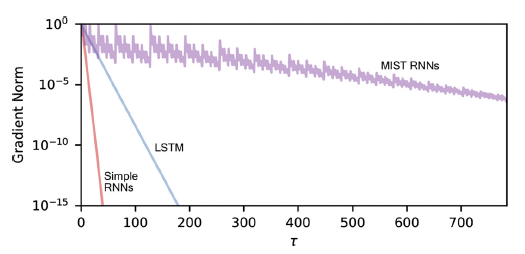
\includegraphics[width=0.8\textwidth]{grad_exp.png}
	\caption{Exponential decrease of the gradient size of a simple RNN (red) or a LSTM (blue) (source: \cite{Teuwen2019}).}
	\label{fig:grad_exp}
\end{figure}


\subsection{LSTM}\label{s:LSTM}

\begin{figure}[ht]
	\centering
	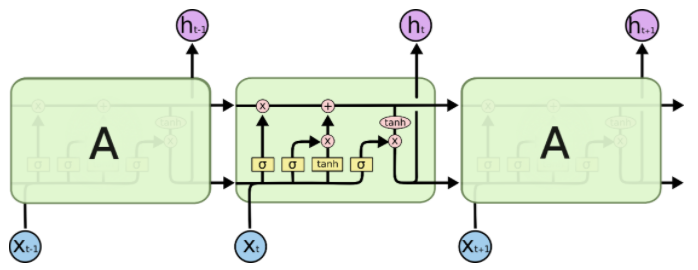
\includegraphics[width=1.0\textwidth]{LSTM_cell.png}
	\caption{A LSTM cell that is repeated over time (source: \cite{Olah}).}
	\label{fig:LSTM_cell}
\end{figure}

As discussed in Section \ref{s:Problems} the LSTM is an updated version of the conventional RNN first proposed by \textbf{Hochreiter \& Schmidhuber} in $ 1997 $ to deal with the short term memory it suffers from. A LSTM can longer take important aspects of the presented time series into account while outputting a current prediction. To do this a LSTM makes use of three gates: forget gate $ \textbf{f}_t $, input gate $ \textbf{i}_t $ and an output gate $ \textbf{o}_t $. When comparing the three gates with equation \ref{eq:RNN}, it is clear that every gate is by itself a recurrent neural network, with the only difference that a sigmoid function is used instead of a hyperbolic tangent. The core concept of the LSTM is that it makes use of a memory cell that is passed on through the different time steps. The memory cell contains important information that is seen before in the data and should be taken into account at the current new output. The three gates can delete, write and read information from this memory cell. It can also be noted that equation \ref{LSTM_rnn} is exactly equal to the conventional RNN described by equation \ref{eq:RNN}. Equation \ref{LSTM_rnn} processes the hidden states $ H_t $ and the new input $ X_t $ to propose an update $ \tilde{\textbf{c}}_t $ to the previous memory cell. The input gate (Eq. \ref{LSTM_input}) decides what will be preserved of the proposal and actually updated. The forget gate (Eq. \ref{LSTM_forget}) decides what will be preserved from the original memory cell $ \textbf{c}_t $. When both the old memory cell and the proposal are pruned, they are combined to one new memory cell. This new memory cell is together with the output gate (Eq. \ref{LSTM_output}) used to output new hidden states. \\

In order to train a LSTM neural network there are considerably more parameters that have to be learned. There are now four different weight matrices for both the hidden states and the inputs. Because by this increase of weights also the expressiveness of the model has increased with respect to the vanilla recurrent neural network of Section \ref{s:RNN}. Therefore, overfitting of the data should be extra monitored. Further, it can also be noted when looking to the LSTM equations that when the parameter that determines the amount of hidden states this will have a higher effect on the calculation load of a LSTM than the vanilla RNN. This is similar when more inputs are added.


The LSTM equations are given as follows as they were found in \cite{Teuwen2019}:
\begin{equation}\label{LSTM_forget}
	\textbf{f}_{t} = \sigma(\textbf{W}_{fH}\textbf{H}_{t-1}+\textbf{W}_{fX}\textbf{X}_{t-1}+\textbf{b}_{f}),
\end{equation}
\begin{equation}\label{LSTM_input}
	\textbf{i}_{t} = \sigma(\textbf{W}_{iH}\textbf{H}_{t-1}+\textbf{W}_{iX}\textbf{X}_{t-1}+\textbf{b}_{i}),
\end{equation}
\begin{equation}\label{LSTM_output}
	\textbf{o}_{t} = \sigma(\textbf{W}_{oH}\textbf{H}_{t-1}+\textbf{W}_{oX}\textbf{X}_{t-1}+\textbf{b}_{o}),
\end{equation}
\begin{equation}\label{LSTM_rnn}
	\tilde{\textbf{c}}_{t} = \tanh(\textbf{W}_{cH}\textbf{H}_{t-1}+\textbf{W}_{cX}\textbf{X}_{t-1}+\textbf{b}_{c}),
\end{equation}
\begin{equation}\label{LSTM_memory}
	\textbf{c}_t = \textbf{f}_t\times\textbf{c}_{t-1}+\textbf{i}_t\times\tilde{\textbf{c}}_t,
\end{equation}
\begin{equation}\label{LSTM_next}
	\textbf{H}_t = \textbf{o}_t\times\tanh(\textbf{c}_t).
\end{equation}


\subsection{GRU}\label{s:GRU}

\begin{figure}[ht]
	\centering
	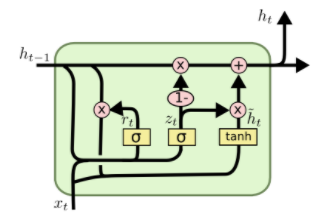
\includegraphics[width=0.6\textwidth]{GRU_cell.png}
	\caption{A GRU cell that is repeated over time (source: \cite{Olah}).}
	\label{fig:GRU_cell}
\end{figure}

Gated 

% Gated recurrent units
add here some information about gru --> one note
%Gated recurrent units (GRUs) [10] were later introduced as a simpler alternative to
%LSTM, and have also become quite popular.
There many different versions of the LSTM and GRU implementations. It has been shown in in [21](see paper), that the performance of are all similar. 

% GRUs are simpler than LSTM, as they use one less gate and eliminate the concept of a seperate cell and hidden state
the need for distinguishing between hidden states and memory cells.

The GRU equations are given as follows as was found in \cite{Teuwen2019}:
Which of these variants is best? Do the differences matter? Greff, et al. (2015) 

\begin{equation}
	\textbf{z}_{t} = \sigma(\textbf{W}_{zH}\textbf{H}_{t-1}+\textbf{W}_{zX}\textbf{X}_{t-1}+\textbf{b}_{z}),
\end{equation}
\begin{equation}
	\textbf{r}_{t} = \sigma(\textbf{W}_{rH}\textbf{H}_{t-1}+\textbf{W}_{rX}\textbf{X}_{t-1}+\textbf{b}_{r}),
\end{equation}
\begin{equation}
	\tilde{\textbf{H}}_{t}=\tanh(\textbf{W}_{HH}(\textbf{r}_t\times\textbf{H}_{t-1})+\textbf{W}_{HX}\textbf{X}_t+\textbf{b}_H),
\end{equation}
\begin{equation}
	\textbf{H}_t=\textbf{z}_t\times\textbf{H}_{t-1}+(1-\textbf{z}_t)\times\tilde{\textbf{H}}_t.
\end{equation}



%chrome-extension://dagcmkpagjlhakfdhnbomgmjdpkdklff/enhanced-reader.html?openApp&pdf=https%3A%2F%2Farxiv.org%2Fpdf%2F1412.3555.pdf


\section{Short-Term residential electrical load forecasting}
\textbf{Pooling paper}
%Things should get out of paper:
%Problem that was solved.
%Method
%Result
Classical ways to deal with uncertainty.\\
Residential electrical load series have a high amount of volatility and uncertainty due to the contingency of the electrical consumption. Classical ways to deal with this are discussed in \cite{Shi2018} and listed as follows:
\begin{enumerate}
	\item Clustering to group similar houses based on historic load or exogenous consumption driving variables. Because the load or driving variables are similar in a cluster, the variance of uncertainty is also decreased. However, performance is very dependent of the dataset. \textbf{But the uncertainty on the whole is reduced --> on single household stays the same!!}
	\item Aggregating the residential loads to cancel out the uncertainties. The aggregated signal will show more regular patterns which means that is easier to predict.The downside is that the aggregated forecast will do a poor job of serving as forecast for a household
	\item A spectral analysis e.g. wavelet analysis, Fourier transforms and empirical mode decomposition aim at seperating a load serie into a regular pattern, an uncertain signal and noise. Because the amount of regularity is low in a residential load serie, this method is infeasible.
\end{enumerate}



In this paper \cite{Shi2018} a novel pooling-based deep recurrent neural network is proposed which collects load profiles of neighbouring houses into a pool of training inputs. Pooling of neighbouring households historical loads to serve as input of the ``Deep Recurrent Neural Network'', is proposed to increase the data volume and diversity of load forecasting, which mitigates the effect of overfitting present in a DRNN. The idea is as quoted by \cite{Shi2018} to use the interconnected spacial information to compensate insufficient temporal information.Thereby, the pool of data allows to learn the correlations between neighbouring households and the shared uncertainties coming from external factors e.g. temperature.  Also, due to the pooling of different households during training the DRNN is able to learn common uncertainties. In paper \cite{Shi2018} pools consisting of $ 10 $ households are used. From the pool of inputs every epoch a randomly chosen batch of load signals are fed to the network. LSTM is applied to mittigate the short term memory of the RNN. Additionally, there is been made use of early stopping to further avoid overfitting. To implement early stopping there has been looked at the ``MSE'' for k iterations, obtained by cross-validation. When the variance of this sequence gets smaller than a specified variable, training stops. When the training ends, performance is tested on each household by using the learned network to perform a feed-forward prediction of the electrical load.\\

An overview of the different steps that were done during the proposed method are: data cleaning and preprocessing $\rightarrow$ data pooling $\rightarrow$ data sampling $\rightarrow$ data training $\rightarrow$ benchmarking.\\

Performance of the proposed method was finally evaluated based on a test set of the last $ 30 $ days and consisting out of : 
\begin{enumerate}
	\item performance of the proposed method with respect to Vanilla RNN, SVR and DRNN (without pooling)
	\item the effect of the neural network depth and pooling
\end{enumerate}

The proposed DRNN with pooling outperforms all other four methods based on following three metrics:

\begin{equation}\label{eq:RMSE}
	RMSE = \sqrt{\frac{\sum_{t=1}^{N}(\hat{y}_t-y_t)^2}{N}}
\end{equation}
\begin{equation}\label{eq:NRMSE}
	NRMSE = \frac{RMSE}{y_{max}-y_{min}}
\end{equation}
\begin{equation}\label{eq:MAE}
	MAE = \frac{\sum_{t=1}^{N}\abs{\hat{y}_t-y_t}}{N}
\end{equation}
\textbf{Actually LSTM network}
The amount of which the PDRNN outperformed the other methods can be seen in Table \ref{tab:pooling_result}. The effect of the depth of the DRNN and the pooling method is depicted in Figure \ref{fig:Shi2018_result}. It can be seen that without the pooling method the DRNN only benefits from extra layers till three are used. This is because from that point, overfitting will reduce the generalization capacity of the DRNN. With the pooling technique, extra layers stays beneficial. It can thus be concluded that introducing extra hidden layers is a good choice to model the non-linear relations, but this can only be done efficiently when overfitting is mittigated by the use of a pooling strategy.The RNN with pooling used for benchmarking consisted out of five layers and thirty hidden units in each layer.

\begin{figure}[h!]
	\centering
	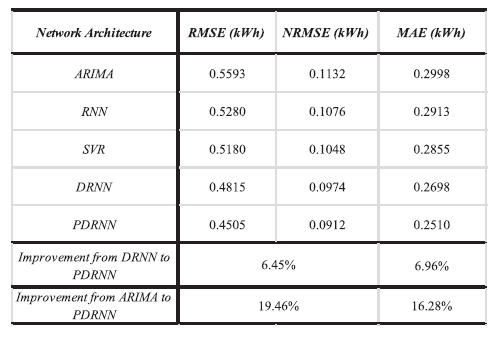
\includegraphics[width=1\textwidth]{pooling_result.png}
	\caption{Results obtained in paper \cite{Shi2018} using the PDRNN method.}
	\label{fig:Shi2018_result}
\end{figure}

\begin{figure}[h!]
	\centering
	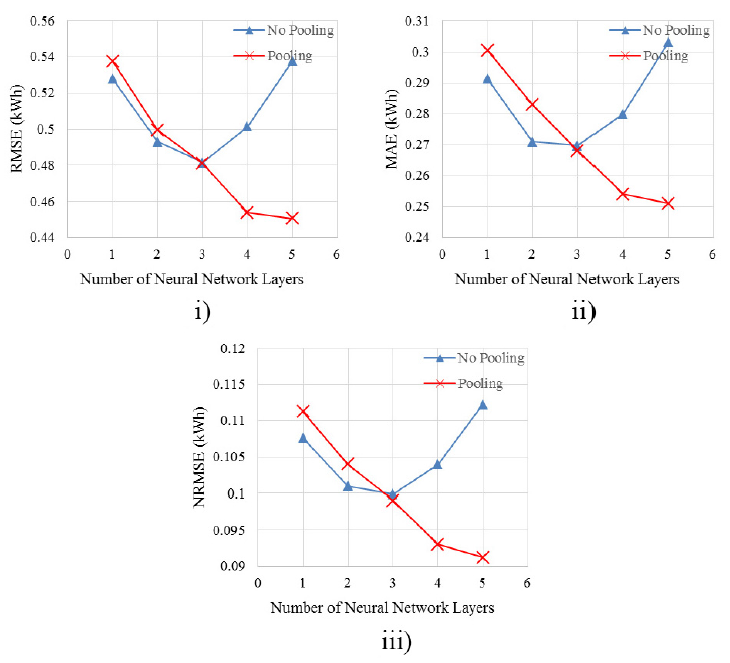
\includegraphics[width=1\textwidth]{Shi2018_result.png}
	\caption{Influence of the number of layers and the pooling method used in \cite{Shi2018}.}
	\label{fig:Shi2018_result}
\end{figure}

GRU (Gated Reset Update) or LSTM (Long Short Term Memory) can be implemented. They are both enhancements of the vanilla RNN which suffers from a vanishing gradient which causes it to to behave without a long term memory. In practise to know which one works often both are tried \cite{Teuwen2019}. Stochastic gradient descent means that the approximated gradient is calculated from a random subset of the available data instead from the entire dataset. \\

\textbf{Short-term Residential load forecasting based on LSTM RNN paper}\\
In \cite{Kong2019} it is chosen for a LSTM approach to forecast the complex temporal consumption pattern which characterises a single household electricity load. It is discussed that the diversity in the aggregated level of the individual electrical loads, smooths the daily load profile. This has as effect that the aggregated electrical load time-serie becomes more predictable, while a single household electrical load is more dependent on the human behaviour of its residents. This is substantiated by making use of a density based clustering technique where it was shown that the different daily consumptions of the aggregated signal could be described by one cluster and no outliers. An outlier means that a daily consumption could not be assigned to a cluster. On the other hand for individual time series the amount of outliers could range to over $ 80 $. To compare the consistency of different individual load signals the amount of outliers could therefore be used.\\
Because the residents daily routine is characterizing the household load so much, this is tried to be learned directly inside the LSTM RNN.\\
Inputs that are given to the LSTM are k past half hour load measurements, the time of when this measurements were taken, the day of the week of the measurements and if this day is a holiday or not. In table \ref{tab:LSTM_lit_result} the results are shown of the LSTM RNN method in comparison with other forecasting techniques. It can be noted that the proposed technique outperforms the rest based on the average performance of $ 29,808 $ individual forecasts of half an hour individual loads. Forecasting was performed on $ 69 $ different electrical loads coming from households in Australia.  However, for individual load series forecasting the MAPE minimization is also remarkable when considering its simplicity in comparison with LSTM. Next, it was concluded that learning methods that had good performance on aggregated time-series e.g. IS-HF and KNN, perform much worse when predicting individual loads. \\
Further, by making use of a regresion technique in function of the amount of outliers it is shown that LSTM and BPNN (Back-Propagation Neural Network) perform similar for, as previously discussed, consistent individual loads. The LSTM only starts to differentiate in performance when inconsistency grows. To conclude things that lack in \cite{Kong2019} are practical useful forecasts of a timespan of $ 24 $h instead of only half an hour and making use of a rule of thumb when parameter tuning. Hyperparameters that can be tuned in LSTM are: learning rate, lag variable, amount of hidden layers and the amount of hidden nodes.\\

\begin{figure}[h!]
	\centering
	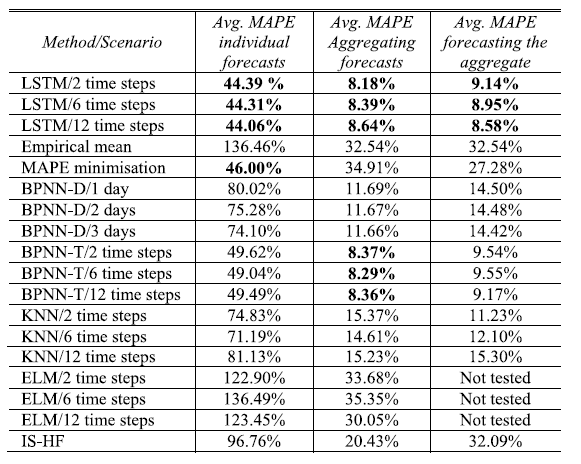
\includegraphics[width=1\textwidth]{prev_appr.png}
	\caption{Different approaches tried in \cite{Kong2019} and their averaged performance of $ 29,808 $ individual forecasts of half an hour individual loads. }
	\label{tab:LSTM_lit_result}
\end{figure}

\textbf{CNN-LSTM paper}\\
In \cite{Kim2019} a novel technique is proposed which makes use of a convolutional neural network from which the outputs are given to a LSTM recurrent network after which a fully connected neural network  is used to produce the outputs. The purpose of the CNN is to extract the features that are the main drivers of energy consumption and to remove the noise that comes initially together with the raw inputs. The CNN is made up out of convolution layers and pooling layers and makes use of the ``ReLU'' activation function. The main purpose of a convolution layer is to extract features while the pooling layer reduces the number of parameters by making use of the ``max pooling principle''. Using the ``max pooling principle'' means taking the max value of each neuron cluster of the previous layer. As discussed in paper \cite{Kong2019} LSTM is suitable to alleviate the problem of a vanishing or exploding gradient which characterized a simple RNN. LSTM is able to preserve long-term memory by making use of memory states that is used in the calculation of hidden states. It is therefore suitable to remembering the irregular trend of the electrical load time-serie. Finally, a fully connected time-serie predicts the load forecast.\\
Paper \cite{Kim2019} further showed superiority with respect to only making use of the LSTM layers as can be seen in Table \ref{tab:CNN-LSTM_results}. The  Inputs that were used to forecast the household load which is located in France are: three submeters with historical loads, global intensity, voltage, global reactive power, global active power, time, data and month. 
At last, also an analysis is performed to investigate the influence of the different inputs by calculating the average class activation score over the inputs. The results are shown in Figure \ref{fig:LSTM-CNN_results}. It can be seen that especially ``Sub metering $ 3 $'' has a big influence on the final forecasts. This sub meter corresponds to the the electric water heater and air conditioner of the house. As was shown in Section \ref{tab:attributes} the dataset used in this thesis gives only information about the presence of a hot water heater.  Discussed limitations in the paper are the definition of the hyper parameters that were set by trail and error instead of using an automated method e.g. a genetic algorithm. A further limitation is the lack of household characteristics e.g. the amount of residents living in the house. It has previously been shown by \textbf{C. Beckel et al.} that household occupancy is one of the primarily drivers of electrical consumption in a household.\\

\begin{figure}[h!]
	\centering
	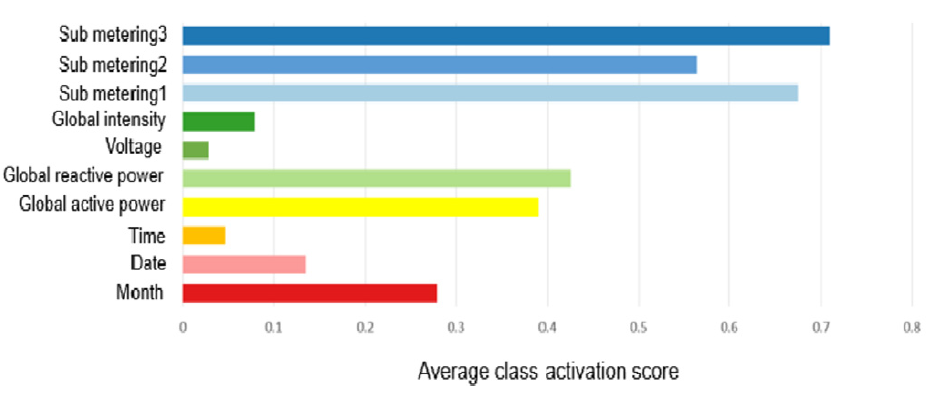
\includegraphics[width=1\textwidth]{CNN-LSTM_results_F.png}
	\caption{The importance of the different inputs as based on the average class activation score. (source \cite{Kim2019})}
	\label{tab:LSTM_lit_results}
\end{figure}

\begin{figure}[h!]
	\centering
	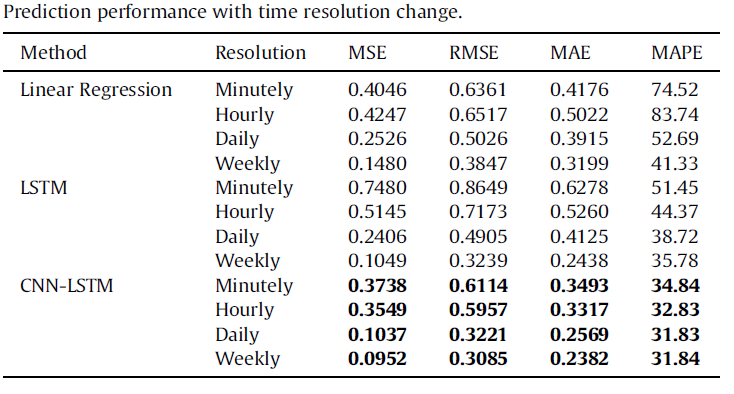
\includegraphics[width=1\textwidth]{CNN-LSTM_results_T.png}
	\caption{Comparison between LSTM and CNN-LSTM. (source: \cite{Kim2019})}
	\label{tab:LSTM_lit_results}
\end{figure}

\textbf{CNN-GRU paper}\\
\cite{Sajjad2020}

\textbf{See oneNote for the summary of the paper and say that it is showed that CNN-GRU performs even better than CNN-LSTM}


%\begin{table}
%  \centering
%  \begin{tabular}{||l|lr||} \hline
%    gnats     & gram      & \$13.65 \\ \cline{2-3}
%              & each      & .01 \\ \hline
%    gnu       & stuffed   & 92.50 \\ \cline{1-1} \cline{3-3}
%    emu       &           & 33.33 \\ \hline
%    armadillo & frozen    & 8.99 \\ \hline
%  \end{tabular}
%  \caption{A table with the wrong layout.}
%  \label{tab:wrong}
%\end{table}
%
%\begin{table}
%  \centering
%  \begin{tabular}{@{}llr@{}} \toprule
%    \multicolumn{2}{c}{Item} \\ \cmidrule(r){1-2}
%    Animal    & Description & Price (\$)\\ \midrule
%    Gnat      & per gram    & 13.65 \\
%              & each        & 0.01 \\
%    Gnu       & stuffed     & 92.50 \\
%    Emu       & stuffed     & 33.33 \\
%    Armadillo & frozen      & 8.99 \\ \bottomrule
%  \end{tabular}
%  \caption{A table with the correct layout.}
%  \label{tab:ok}
%\end{table}



\section{Conclusion}
The final section of the chapter gives an overview of the important results
of this chapter. This implies that the introductory chapter and the
concluding chapter don't need a conclusion.



%%% Local Variables: 
%%% mode: latex
%%% TeX-master: "thesis"
%%% End: 
